% ===============================================================
%  جلسه دهم
% ===============================================================
\chapter{عملگر میانگین‌گیری، واریانس، مُد و میانه}

\section{میانگین‌گیری یا عملگر \lr{Expectation}}

فرض کنید که $X,Y,Z,\ldots$ متغیرهای تصادفی \textcolor{red!70!black}{مستقل} و یا \textcolor{red!70!black}{وابسته} باشند. در این صورت، به ازای یک تابع مشخص $g$، مقدار $g(X,Y,Z,\ldots)$ نیز بدل به یک متغیر تصادفی جدید خواهد شد.

\begin{definition}[میانگین تابعی از چند متغیر]
میانگین و یا \lr{Expectation} تابع $g$ در این شرایط را به صورت زیر تعریف می‌کنیم:
\[
\E\{g(X,Y,Z,\ldots)\}=\sum_{x,y,z,\ldots}g(x,y,z,\ldots)\,\Prob(X=x,\ Y=y,\ Z=z,\ldots).
\]
در صورت پیوسته بودن هر یک از متغیرهای تصادفی $X,Y,Z,\ldots$، به جای \lr{pmf} می‌بایست از \lr{pdf} کلی (توأم) استفاده نمود و جمع را با انتگرال جایگزین کرد:
\[
\E\{g(X,Y,\ldots)\}=\int\!\!\int\cdots g(x,y,\ldots)\,f_{X,Y,\ldots}(x,y,\ldots)\dd x\dd y\cdots
\]
\end{definition}

\begin{itemize}
\item در صورتی که متغیرهای تصادفی \textbf{مستقل} باشند، تابع \lr{pmf} کلی به صورت حاصل‌ضرب توابع \lr{pmf} حاشیه‌ای در خواهد آمد:
$\Prob(X=x,Y=y,\ldots)=\Prob(X=x)\Prob(Y=y)\cdots$.
\item دقت کنید که با میانگین‌گیری یا عمل \lr{Expectation}، به یک مقدار قطعی خواهیم رسید و تمام تصادفی بودن (\lr{Randomness}) از بین می‌رود.
\end{itemize}

\begin{note}
\notetitle به این قاعده گاهی «قانون آماردان ناخودآگاه» (\lr{LOTUS}) می‌گویند: برای محاسبه $\E[g(X)]$ لازم نیست ابتدا توزیع متغیر جدید $g(X)$ را پیدا کنیم؛ کافی است $g$ را روی توزیع خود $X$ میانگین بگیریم.
\end{note}

\begin{example}[میانگین ضرب دو تاس]
دو تاس سالم و مستقل پرتاب می‌شوند. $\E(XY)$ و $\E(\max(X,Y))$ را بیابید.
\begin{solution}
با استقلال، $\Prob(X=x,Y=y)=\frac1{36}$:
$\E(XY)=\frac1{36}\sum_{x=1}^6\sum_{y=1}^6xy=\frac1{36}(21)(21)=\frac{441}{36}=12.25=\E(X)\E(Y)$.

برای ماکزیمم: $\Prob(\max\le m)=\frac{m^2}{36}$، پس $\Prob(\max=m)=\frac{m^2-(m-1)^2}{36}=\frac{2m-1}{36}$ و
$\E(\max)=\frac{1}{36}\sum_{m=1}^6m(2m-1)=\frac{1+6+15+28+45+66}{36}=\frac{161}{36}\approx4.47$.
\end{solution}
\end{example}

\section[واریانس و انحراف معیار]{واریانس و انحراف معیار {\large\lr{(Variance \& Std.\ Deviation)}}}

یکی دیگر از آماره‌های پرکاربرد در آمار و احتمال \textbf{واریانس} یک متغیر تصادفی مانند $X$ است که آن را با $\Var(X)$ نشان می‌دهیم.

\begin{definition}[واریانس و انحراف معیار]
با $\mu=\E(X)$:
\[
\Var(X)=\E\big((X-\mu)^2\big)=\int_{-\infty}^{\infty}(x-\mu)^2f_X(x)\dd x,\qquad
\Var(X)=\sum_x(x-\mu)^2P(X=x),
\]
\[
\sigma(X)=\sqrt{\Var(X)} .
\]
\end{definition}

واریانس، و یا جذر آن «انحراف معیار $\sigma(X)$» میزان \textbf{پراکندگی} یک متغیر تصادفی حول میانگین را نشان می‌دهند. دو توزیع می‌توانند میانگین یکسان (مثلاً ۱۰۰) ولی پراکندگی کاملاً متفاوت داشته باشند:

\begin{center}
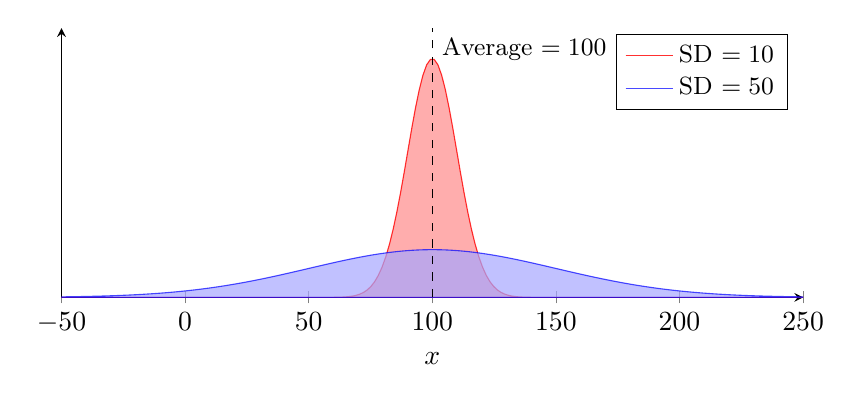
\begin{tikzpicture}
\begin{axis}[width=11cm,height=5cm,axis lines=left,xmin=-50,xmax=250,ymin=0,ymax=0.045,ytick=\empty,xlabel={$x$},samples=200,domain=-50:250,legend style={font=\small}]
\addplot[fill=red!40,draw=red,opacity=0.8] {exp(-(x-100)^2/(2*10^2))/(sqrt(2*pi)*10)} \closedcycle; \addlegendentry{\lr{SD} $=10$}
\addplot[fill=blue!35,draw=blue,opacity=0.7] {exp(-(x-100)^2/(2*50^2))/(sqrt(2*pi)*50)} \closedcycle; \addlegendentry{\lr{SD} $=50$}
\draw[dashed] (axis cs:100,0) -- (axis cs:100,0.045) node[below right,font=\small]{\lr{Average} $=100$};
\end{axis}
\end{tikzpicture}
\end{center}

\begin{note}
\notetitle چرا مربع و نه قدر مطلق؟ $\E|X-\mu|$ (انحراف مطلق میانگین) هم معیار پراکندگی است، اما واریانس خواص جبری بسیار زیباتری دارد (مثلاً جمع‌پذیری برای متغیرهای مستقل، پایین‌تر). انحراف معیار هم‌واحد با $X$ است (مثلاً سانتی‌متر)، اما واریانس واحد مربع دارد.
\end{note}

\subsection{خواص}
\begin{theorem}[خواص واریانس]
فرض کنید $X$ یک متغیر تصادفی پیوسته، گسسته و یا مخلوط باشد و واریانس آن وجود داشته باشد. آنگاه:
\begin{enumerate}
\item همواره داریم:
\[
\Var(X)=\E\big((X-\E(X))^2\big)=\E(X^2)-\E(X)^2\ge0 .
\]
\item در صورتی که $a,b$ اعداد ثابت حقیقی باشند، داریم:
\[
\Var(aX+b)=a^2\Var(X).
\]
\item در صورتی که $X,Y$ متغیرهای تصادفی \textcolor{red!70!black}{مستقل} باشند، داریم:
\[
\E(XY)=\E(X)\E(Y),\qquad \Var(X+Y)=\Var(X)+\Var(Y).
\]
\end{enumerate}
\end{theorem}

\begin{proof}
(۱) با بسط مربع و خاصیت خطی میانگین ($\mu$ یک عدد ثابت است):
\[
\E\big((X-\mu)^2\big)=\E(X^2-2\mu X+\mu^2)=\E(X^2)-2\mu\E(X)+\mu^2=\E(X^2)-\mu^2 .
\]
نامنفی بودن از آنجاست که $(X-\mu)^2\ge0$ (یا از نامساوی جنسن).

(۲) $\E(aX+b)=a\mu+b$؛ پس $aX+b-\E(aX+b)=a(X-\mu)$ و
$\Var(aX+b)=\E\big(a^2(X-\mu)^2\big)=a^2\Var(X)$. (افزودن ثابت $b$ فقط توزیع را جابه‌جا می‌کند و پراکندگی را تغییر نمی‌دهد.)

(۳) \textbf{ضرب:} با استقلال، $\Prob\{X=x,Y=y\}=\Prob\{X=x\}\Prob\{Y=y\}$؛ پس
\[
\begin{aligned}
\E(XY)&=\sum_{x,y}xy\,\Prob\{X=x,Y=y\}=\sum_{x,y}xy\,\Prob\{X=x\}\Prob\{Y=y\}\\
&=\sum_xx\Prob\{X=x\}\sum_yy\Prob\{Y=y\}=\E(X)\E(Y).
\end{aligned}
\]
(در حالت پیوسته روابط مشابهی با انتگرال و $f_{X,Y}=f_Xf_Y$ می‌توان نوشت.)

\textbf{جمع:} با $\mu_X=\E X$ و $\mu_Y=\E Y$:
\[
\begin{aligned}
\Var(X+Y)&=\E\big\{(X+Y-\mu_X-\mu_Y)^2\big\}\\
&=\E\big\{(X-\mu_X)^2+(Y-\mu_Y)^2+2(X-\mu_X)(Y-\mu_Y)\big\}\\
&=\E\big\{(X-\mu_X)^2+(Y-\mu_Y)^2\big\}=\Var(X)+\Var(Y).
\end{aligned}
\]
در سطر سوم از خاصیت خطی بودن عملگر \lr{Expectation} و همچنین نتیجه بند پیشین استفاده شده است: $X-\mu_X$ و $Y-\mu_Y$ مستقل‌اند، پس
$\E\{(X-\mu_X)(Y-\mu_Y)\}=\E(X-\mu_X)\,\E(Y-\mu_Y)=0\times0=0$.
\end{proof}

\begin{warning}
\warntitle بدون استقلال، $\Var(X+Y)=\Var X+\Var Y$ لزوماً درست نیست. مثلاً اگر $Y=X$ آنگاه $\Var(2X)=4\Var X\neq2\Var X$؛ و اگر $Y=-X$ آنگاه $\Var(X+Y)=0$. جمله اضافی $2\E\{(X-\mu_X)(Y-\mu_Y)\}$ همان «کوواریانس» است که در جلسات آینده مطالعه می‌کنیم. همچنین دقت کنید: $\Var(X-Y)=\Var X+\Var Y$ (نه تفاضل!)، زیرا $\Var(-Y)=(-1)^2\Var Y$.
\end{warning}

\section{واریانس توزیع‌های معروف}

\subsection{توزیع‌های برنولی، دوجمله‌ای و پواسون}

\begin{example}[برنولی $X\sim\mathrm{Bern}(p)$]
\[
\begin{aligned}
\Var(X)&=p\times(1-p)^2+(1-p)\times(0-p)^2=p(1-p)\big[(1-p)+p\big]=p(1-p),\\
\sigma(X)&=\sqrt{p(1-p)} .
\end{aligned}
\]
(روش دیگر: $X^2=X$ پس $\E X^2=p$ و $\Var X=p-p^2$.) بیشینه واریانس در $p=\frac12$ رخ می‌دهد: سکه سالم «غیرقابل‌پیش‌بینی‌ترین» است.
\end{example}

\begin{example}[دوجمله‌ای $X\sim\mathrm{Binomial}(n,p)$]
\[
\Var(X)=\sum_{i=0}^{n}(i-np)^2\binom nip^i(1-p)^{n-i}=np(1-p).
\]
\begin{solution}
\textbf{روش سریع:} $X=\sum_{i=1}^nB_i$ که $B_i$ها برنولی‌های مستقل‌اند. طبق خاصیت جمع واریانس برای متغیرهای مستقل: $\Var X=\sum\Var B_i=np(1-p)$.

\textbf{روش مستقیم:} با اتحاد $k(k-1)\binom nk=n(n-1)\binom{n-2}{k-2}$ داریم $\E[X(X-1)]=n(n-1)p^2$. پس
$\E X^2=n(n-1)p^2+np$ و $\Var X=n(n-1)p^2+np-n^2p^2=np-np^2=np(1-p)$.
\end{solution}
\end{example}

\begin{example}[پواسون $X\sim\mathrm{Poisson}(\lambda)$]
\[
\E(X)=\lambda,\qquad \Var(X)=\lambda .
\]
\begin{solution}
$\E[X(X-1)]=\sum_{k\ge2}k(k-1)e^{-\lambda}\frac{\lambda^k}{k!}=\lambda^2e^{-\lambda}\sum_{k\ge2}\frac{\lambda^{k-2}}{(k-2)!}=\lambda^2$. پس $\E X^2=\lambda^2+\lambda$ و $\Var X=\lambda^2+\lambda-\lambda^2=\lambda$. (سازگار با حد دوجمله‌ای: $np(1-p)\to\lambda$ وقتی $p\to0$.)
\end{solution}
\end{example}

\subsection{توزیع‌های گاوسی، نمایی و یکنواخت}

\begin{example}[گاوسی $X\sim\mathcal N(\mu,\sigma^2)$]
$\Var(X)=\sigma^2$.
\begin{solution}
با $z=\frac{x-\mu}{\sigma}$: $\Var X=\sigma^2\int z^2\frac{e^{-z^2/2}}{\sqrt{2\pi}}\dd z$. با انتگرال‌گیری جزءبه‌جزء ($u=z$، $\dd v=ze^{-z^2/2}\dd z$):
$\int z^2e^{-z^2/2}\dd z=\big[-ze^{-z^2/2}\big]_{-\infty}^{\infty}+\int e^{-z^2/2}\dd z=\sqrt{2\pi}$. پس $\Var X=\sigma^2$ ــ پارامتر $\sigma^2$ دقیقاً همان واریانس است.
\end{solution}
\end{example}

\begin{example}[نمایی $X\sim\mathrm{Exponential}(\lambda)$]
\[
\Var(X)=\lambda\int_0^\infty\big(x-\lambda^{-1}\big)^2e^{-\lambda x}\dd x=\lambda^{-2}.
\]
\begin{solution}
با $\int_0^\infty x^ne^{-\lambda x}\dd x=\frac{n!}{\lambda^{n+1}}$: $\E X^2=\lambda\cdot\frac{2}{\lambda^3}=\frac{2}{\lambda^2}$. پس $\Var X=\frac2{\lambda^2}-\frac1{\lambda^2}=\frac{1}{\lambda^2}$؛ یعنی $\sigma=\E X=\frac1\lambda$.
\end{solution}
\end{example}

\begin{example}[یکنواخت $X\sim\mathrm{Uniform}(a,b)$]
\[
\Var(X)=\frac{1}{12}(b-a)^2 .
\]
\begin{solution}
$Y=X-\frac{a+b}{2}$ روی $[-\frac L2,\frac L2]$ یکنواخت است ($L=b-a$). پس
$\Var X=\E Y^2=\frac1L\int_{-L/2}^{L/2}y^2\dd y=\frac1L\cdot\frac{2}{3}\Big(\frac L2\Big)^3=\frac{L^2}{12}$.
\end{solution}
\end{example}

\begin{summarybox}[جدول خلاصه میانگین و واریانس توزیع‌های معروف]
\centering
\renewcommand{\arraystretch}{1.5}
\begin{tabular}{l|c|c}
توزیع & $\E(X)$ & $\Var(X)$\\\hline
برنولی $\mathrm{Bern}(p)$ & $p$ & $p(1-p)$\\
دوجمله‌ای $\mathrm{Bin}(n,p)$ & $np$ & $np(1-p)$\\
هندسی (احتمال موفقیت $p$) & $\frac1p$ & $\frac{1-p}{p^2}$\\
پواسون $\mathrm{Pois}(\lambda)$ & $\lambda$ & $\lambda$\\
یکنواخت $\mathcal U(a,b)$ & $\frac{a+b}2$ & $\frac{(b-a)^2}{12}$\\
نمایی $\mathrm{Exp}(\lambda)$ & $\frac1\lambda$ & $\frac1{\lambda^2}$\\
گاوسی $\mathcal N(\mu,\sigma^2)$ & $\mu$ & $\sigma^2$\\
لاپلاس $(\mu,b)$ & $\mu$ & $2b^2$\\
بتا $(\alpha,\beta)$ & $\frac{\alpha}{\alpha+\beta}$ & $\frac{\alpha\beta}{(\alpha+\beta)^2(\alpha+\beta+1)}$\\
کوشی & ندارد & ندارد
\end{tabular}
\end{summarybox}

\section{واریانس جمع متغیرهای تصادفی \lr{i.i.d.}}

فرض کنید که $X_1,X_2,\ldots,X_n$ متغیرهای تصادفی \lr{i.i.d.} از یک توزیع با میانگین $\mu$ و واریانس $\sigma^2$ باشند. متغیر تصادفی $\bar X_n$ را به صورت زیر تعریف می‌کنیم:
\[
\bar X_n\triangleq\frac{X_1+X_2+\cdots+X_n}{n}.
\]
در این صورت (با خاصیت جمع‌پذیری واریانس برای متغیرهای مستقل و $\Var(aX)=a^2\Var X$) داریم:
\[
\boxed{\ \Var(\bar X_n)=\sum_{i=1}^{n}\Var\Big(\frac{X_i}{n}\Big)=\sum_{i=1}^{n}\frac{\sigma^2}{n^2}=\frac{\sigma^2}{n}\ }
\]
با افزایش مجانبی $n$، واریانس متغیر تصادفی $\bar X_n$ به سمت صفر میل می‌کند. پس انحراف معیار میانگین نمونه‌ای $\frac{\sigma}{\sqrt n}$ است: برای نصف کردن خطا، باید چهار برابر نمونه جمع کنیم.

\begin{note}
\notetitle این نتیجه، شهود قانون اعداد بزرگ است: $\E\bar X_n=\mu$ و پراکندگی $\bar X_n$ حول $\mu$ به صفر میل می‌کند. در جلسه بعد با «نامساوی چبیشف» همین را به اثبات دقیق شکل ضعیف قانون اعداد بزرگ تبدیل می‌کنیم:
$\Prob(|\bar X_n-\mu|>\varepsilon)\le\frac{\sigma^2}{n\varepsilon^2}\to0$. این همچنین توضیح می‌دهد که چرا در جلسه سوم عرض توزیع تعداد شیرها $O(\sqrt n)$ بود: $\sigma(\text{تعداد شیر})=\sqrt{n/4}$.
\end{note}

\section{مُد و میانه \lr{(Mode and Median)}}

\subsection{مُد \lr{(Mode)}}
\begin{definition}[مد]
به \textcolor{red!70!black}{محتمل‌ترین} مقدار یک متغیر تصادفی، مُد (\lr{Mode}) آن متغیر تصادفی اطلاق می‌گردد: برای متغیر گسسته، مقداری که \lr{PMF} را بیشینه می‌کند؛ برای متغیر پیوسته، نقطه بیشینه \lr{PDF}.
\end{definition}
مثال: اگر $P(X=1)=0.2$، $P(X=3)=0.5$ و $P(X=7)=0.3$ آنگاه مد برابر ۳ است (در حالی که میانگین $0.2+1.5+2.1=3.8$ است).

\begin{center}
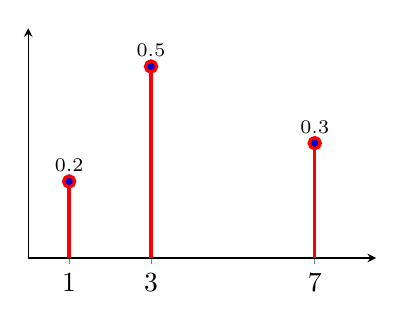
\begin{tikzpicture}
\begin{axis}[width=6cm,height=4.5cm,axis lines=middle,xmin=0,xmax=8.5,ymin=0,ymax=0.6,xtick={1,3,7},ytick=\empty]
\addplot+[ycomb,very thick,red,mark=*] coordinates {(1,0.2) (3,0.5) (7,0.3)};
\node[above,font=\scriptsize] at (axis cs:1,0.2) {$0.2$};
\node[above,font=\scriptsize] at (axis cs:3,0.5) {$0.5$};
\node[above,font=\scriptsize] at (axis cs:7,0.3) {$0.3$};
\end{axis}
\end{tikzpicture}
\hspace{4mm}
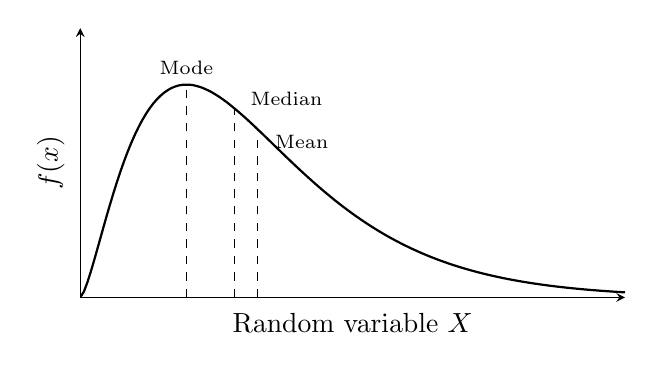
\begin{tikzpicture}
\begin{axis}[width=8.5cm,height=5cm,axis lines=left,xmin=0,xmax=10,ymin=0,ymax=0.3,xtick=\empty,ytick=\empty,xlabel={\lr{Random variable} $X$},ylabel={$f(x)$},samples=150,domain=0:10]
\addplot[black,thick] {x^1.5*exp(-x/1.3)/2.5615};
\draw[dashed] (axis cs:1.95,0) -- (axis cs:1.95,0.237) node[above,font=\scriptsize]{\lr{Mode}};
\draw[dashed] (axis cs:2.83,0) -- (axis cs:2.83,0.211);
\node[font=\scriptsize,anchor=west] at (axis cs:2.95,0.221) {\lr{Median}};
\draw[dashed] (axis cs:3.25,0) -- (axis cs:3.25,0.188);
\node[font=\scriptsize,anchor=west] at (axis cs:3.4,0.173) {\lr{Mean}};
\end{axis}
\end{tikzpicture}
\end{center}

\subsection{میانه \lr{(Median)}}
\begin{definition}[میانه]
میانه به کوچک‌ترین مقداری اطلاق می‌گردد که یک متغیر تصادفی با احتمال $\frac12$ کوچک‌تر یا مساوی آن است. به صورت معادل، به کوچک‌ترین مقداری اطلاق می‌گردد که تابع \lr{CDF} در آن برابر یا بزرگ‌تر یا مساوی $\frac12$ است:
\[
m=\min\{x:\ F_X(x)\ge\tfrac12\}.
\]
\end{definition}
برای متغیر پیوسته، میانه نقطه‌ای است که مساحت زیر \lr{PDF} را به دو نیمه ۵۰٪ تقسیم می‌کند؛ در حالی که میانگین «نقطه تعادل» (مرکز جرم) است.

\begin{note}
\notetitle \textbf{رابطه مد، میانه و میانگین:} برای توزیع‌های متقارن تک‌قله (مانند گاوسی) هر سه برابرند. برای توزیع‌های چوله به راست (دم بلند در سمت راست، مانند نمایی یا توزیع درآمد) معمولاً $\text{مد}<\text{میانه}<\text{میانگین}$؛ زیرا مقادیر بزرگ دم، میانگین را به سمت خود می‌کشند. میانه نسبت به داده‌های پرت «مقاوم» (\lr{robust}) است و حتی برای کوشی (که میانگین ندارد) وجود دارد و برابر $x_0$ است.
\end{note}

\begin{example}[مد، میانه و میانگین توزیع نمایی]
برای $X\sim\mathrm{Exp}(\lambda)$: مد $=0$ (چگالی نزولی است)، میانه از $1-e^{-\lambda m}=\frac12$ برابر $m=\frac{\ln2}{\lambda}\approx\frac{0.693}{\lambda}$ و میانگین $\frac1\lambda$. پس $0<0.693/\lambda<1/\lambda$ ــ مطابق ترتیب توزیع‌های چوله به راست.
\end{example}

\section{تمرین‌های تکمیلی}

\begin{exercise}
واریانس عدد یک تاس سالم را حساب کنید. سپس واریانس مجموع اعداد ۱۰ تاس مستقل را بیابید.
\end{exercise}
\begin{solution}
$\E X=3.5$ و $\E X^2=\frac{91}{6}$؛ پس $\Var X=\frac{91}{6}-\frac{49}{4}=\frac{182-147}{12}=\frac{35}{12}\approx2.92$. برای مجموع ۱۰ تاس مستقل: $10\times\frac{35}{12}=\frac{350}{12}\approx29.17$ (انحراف معیار حدود $5.4$ حول میانگین $35$).
\end{solution}

\begin{exercise}
اگر $\E X=2$ و $\Var X=3$ باشد، $\E[(2X-1)^2]$ و $\Var(5-3X)$ را بیابید.
\end{exercise}
\begin{solution}
$\E X^2=\Var X+(\E X)^2=7$. پس $\E[(2X-1)^2]=4\E X^2-4\E X+1=28-8+1=21$.
$\Var(5-3X)=9\Var X=27$.
\end{solution}

\begin{exercise}
برای اندازه‌گیری یک کمیت، از دستگاهی با خطای تصادفی با انحراف معیار ۲ میلی‌متر استفاده می‌کنیم. چند اندازه‌گیری مستقل لازم است تا انحراف معیار میانگین اندازه‌گیری‌ها حداکثر $0.25$ میلی‌متر شود؟
\end{exercise}
\begin{solution}
$\sigma(\bar X_n)=\frac{2}{\sqrt n}\le0.25\Rightarrow\sqrt n\ge8\Rightarrow n\ge64$.
\end{solution}

\begin{exercise}
میانه و مد توزیع $f(x)=2x$ روی $[0,1]$ را بیابید و با میانگین ($\frac23$) مقایسه کنید.
\end{exercise}
\begin{solution}
$F(x)=x^2$؛ میانه: $m^2=\frac12\Rightarrow m=\frac1{\sqrt2}\approx0.707$. مد: $x=1$ (چگالی صعودی است). ترتیب: $\text{میانگین}=0.667<\text{میانه}=0.707<\text{مد}=1$ ــ این توزیع چوله به چپ است و ترتیب برعکس می‌شود.
\end{solution}
